\begin{tldrbox}
    I can work with pictures instead of sets. I suspect it will be easier for me to spot patterns from pictures rather than set builder notation.
\end{tldrbox}

\subsection{Partitions and Numerical Sets}

This material is background but its worth recalling it here. There exists a bijection
\[\varphi: \textsf{Numerical Sets} \to \textsf{Partitions}\]

constructed by forming walks where each step is decided by an elements membership in a numerical set. A formal construction could look something like this:
\[e_T: \N_{\le \frob(T)} \to \{\rightarrow, \uparrow\}^{\frob(T) + 1}\]

\[e_T(x): \begin{cases} \rightarrow & x \in T \\ \uparrow & x \not\in T\end{cases}\]

but the description of the construction is up to personal preference.

The set \(\Gamma_T := \{(x, e_T(x)): x \in \N_{\le \frob(T)}\}\) describes a walk which is equivalent to the profile of a partition\footnote{The walk is finite because after \(\frob(T)\) every step is a right step. We cut the walk off at this point}. The correspondence \(T \sim_\varphi \Gamma_T\) gives a bijection between numerical sets and partitions. The details can be found in \cite{Constantin2017}. The following is a worked example for constructing a partition from a numerical set.

\begin{examplebox}
    Let \(T\) be the numerical set defined by \(\N_0 \setminus T = \{1, 2, 4\}\) so that \(\frob(T) = 4\). We construct the walk by finding the steps associated to each element less than or equal to \(\frob(T) = 4\).

    \begin{center}
        \begin{tabular}{c|c}
        Element & Step \\
        \hline
        \(0\) & \(\rightarrow\)  \\
        \(1\) & \(\uparrow\) \\
        \(2\) & \(\uparrow\) \\
        \(3\) & \(\rightarrow\) \\
        \(4\) & \(\uparrow\) \\
        \end{tabular}
    \end{center}

    Starting at \(0\) and taking each step gives the following walk:
        \begin{center}
    \begin{center}
    \begin{tikzpicture}[scale=1, >=Stealth]

    % Draw the grid
    \draw[very thin, gray] (0,0) grid (5,3);

    % Draw the axes
    \draw[->] (0,0) -- (5.5,0) node[right] {x};
    \draw[->] (0,0) -- (0,3.5) node[above] {y};

    % Draw the path
    \draw[->, thick] (0,0) -- (1,0) node[midway, below] {\(0\)};
    \draw[->, thick] (1,0) -- (1,1) node[midway, right] {\(1\)};
    \draw[->, thick] (1,1) -- (1,2) node[midway, right] {\(2\)};
    \draw[->, thick] (1,2) -- (2,2) node[midway, below] {\(3\)};
    \draw[->, thick] (2,2) -- (2,3) node[midway, right] {\(4\)};

    % Remove the tick labels on x and y axes
    \foreach \x in {0, 1, 2, 3, 4, 5}
        \draw (\x, 0) -- (\x, -0.1);

    \foreach \y in {0, 1, 2, 3}
        \draw (0, \y) -- (-0.1, \y);

    \end{tikzpicture}
    \end{center}
    \end{center}

    This region to the left of the walk is the partition \(2 + 1 + 1\) which corresponds to the following Ferrers diagram: {\tiny \ydiagram[*(white) ]{2, 1, 1}}. From now on we will omit the arrow heads on the steps of the walk since arrow heads communicate no additional information.
\end{examplebox}

The hook lengths of the partition encode information about the walk and therefore the numerical set associated to the walk. We use \(\lambda(T)\) to denote the partition associated to a numerical set \(T\). It is useful to state some computational tricks.

\subsection{Computational Tricks Using Hooks}

Given a labeled walk, which amounts to a function \(e_T\), we can find the hook lengths by noting each box uniquely determines a right step and an up step.

\begin{center}
    \begin{minipage}{0.5\textwidth}
        \centering
        \begin{tikzpicture}[scale=1, >=Stealth]

        % Draw the grid
        \draw[very thin, gray] (0,0) grid (8,4);

        % Draw the axes
        \draw[->] (0,0) -- (8.5,0) node[right] {x};
        \draw[->] (0,0) -- (0,4.5) node[above] {y};

        % Draw the path
        \draw[thick] (0,0) -- (1,0) node[midway, below] {\(0\)};
        \draw[thick] (1,0) -- (1,1) node[midway, right] {\(1\)};
        \draw[thick] (1,1) -- (2,1) node[midway, below] {\(\textcolor{gray}{2}\)};
        \draw[thick] (2,1) -- (3,1) node[midway, below] {\(3\)};
        \draw[thick] (3,1) -- (3,2) node[midway, right] {\(4\)};
        \draw[thick] (3,2) -- (3,3) node[midway, right] {\(\textcolor{gray}{5}\)};
        \draw[thick] (3,3) -- (4,3) node[midway, below] {\(6\)};
        \draw[thick] (4,3) -- (4,4) node[midway, right] {\(7\)};

        % Remove the tick labels on x and y axes
        \foreach \x in {0, 1, 2, 3, 4, 5, 6, 7, 8}
            \draw (\x, 0) -- (\x, -0.1);

        \foreach \y in {0, 1, 2, 3, 4}
            \draw (0, \y) -- (-0.1, \y);

        % Draw the hook in the box with center (1.5, 2.5)
        \draw[gray, thick] (1.5, 2.5) -- (2.5, 2.5); % Blue line extending to the center of the box to the right
        \draw[gray, thick] (1.5, 2.5) -- (1.5, 1.5); % Blue line going down to the center of the box below
        \fill[blue] (1.5, 2.5) circle (0.2); % Filled blue circle in the middle of the specified box

        \end{tikzpicture}
    \end{minipage}%
    \begin{minipage}{0.5\textwidth}
        \centering
        {\Large \ytableausetup{centertableaux}
        \begin{ytableau}
            7 & 5 & 4 & 1 \\
            6 & *(lightgray) \textcolor{blue}{3} & *(lightgray) 2 \\
            4 & *(lightgray) 2 & 1 \\
            1 \\
        \end{ytableau}}
    \end{minipage}
\end{center}

The length of the hook can be be found be taking the index of the up step (at the right of the arm) the index of the right step (at the bottom of the leg). In the diagram above the blue hook length is \(\textcolor{gray}{5} - \textcolor{gray}{2} = \textcolor{blue}{3}\). Recall that the length of the hook is also the number of boxes the hook crosses. 

\begin{observationbox}
    If \(f\) is a gap of a numerical set \(T\) then \(f\) appears as a hook length in \(\lambda(T)\).
    Each gap of \(T\) appears as an up step in the profile of \(\lambda(T)\) so \(f\) must appear as an up step. By our method for computing the hook lengths described above, the hook length with arm intersecting \(f\) and leg intersecting \(0\) is \(f - 0 = f\). As a remark, it is helpful to note that this hook length is in the leftmost column.
\end{observationbox}

However, thinking in terms of the step indices helps us understand what each box can tell us about the numerical set associated to the walk.

\begin{itemize}
    \item The leftmost column contains all the indices which are up steps. Therefore the leftmost column has exactly the gaps of the numerical set as its hook lengths.
    \item The topmost row contains hook lengths of the form \(\frob(T) - x\) for each \(x \in T\). The void \(M(T)\) contains the elements in the leftmost column that do not appear in the topmost column. We can also find all small elements of \(T\) by taking subtracting the top row hook lengths from \(F(T)\).
\end{itemize}

\begin{examplebox}
    Consider the numerical set \(T\) defined by \(\N_0 \setminus T = \{1, 4, 5, 7\}\) which has the following partition:
    \begin{center}
    \begin{minipage}{0.5\textwidth}
        \centering
        {\Large \ytableausetup{centertableaux}
        \begin{ytableau}
            *(lightgray) 7 & 5 & 4 & 1 \\
            *(lightgray) 6 & 3 & 2 \\
            *(lightgray) 4 & 2 & 1 \\
            *(lightgray) 1 \\
        \end{ytableau}}
        \\[1em]
        \textbf{1: Hook lengths}
    \end{minipage}%
    \begin{minipage}{0.5\textwidth}
        \centering
        {\Large \ytableausetup{centertableaux}
        \begin{ytableau}
            *(lightgray) 0 & *(lightgray) 2 & *(lightgray) 3 & *(lightgray) 6 \\
            1 & 4 & 5 \\
            3 & 5 & 6 \\
            6 \\
        \end{ytableau}}
        \\[1em]
        \textbf{2: \(\frob(T)\) minus hook lengths}
    \end{minipage}
    \end{center}

    \begin{enumerate}
        \item The gaps of \(T\) are exactly the hooks in the left most columnn in the left diagram.
        \item The small elements of \(T\) are NOT the hooks in the topmost row in the top diagram. [beacause T is not a numerical semigroup... fix this later]
    \end{enumerate}
    In practice, one does not need to take \(F(S) - x\) since it is sufficient to know the original top row. I can imagine it might be helpful for computing the dual \(T^*\) of the numerical set.
\end{examplebox}

\subsection{The Atom Monoid}
Antokoletz and Miller defined the atom monoid of a numerical set T in \cite{Antokoletz2002} as
\[A(T) := \{x \in \N_0 \ssep x + T \subseteq T\}.\] This is always a numerical semigroup contained in \(T\).

\begin{proposition}
    \(A(T)\) is a numerical semigroup contained in \(T\).
\end{proposition}
\begin{proof}
    We must show that \(A(T)\) is a cofinite submonoid of \(\N_0\) contained in \(T\). For the low hanging fruit, \(A(T)\) contains \(0\) as \(0 + T = T\). For additive closure, if \(x\) and \(y\) are elements of \(A(T)\) then for any \(t \in T\), \((x + y) + t = x + (y + t)\). Now, \(y + t \in T\) so that \(x + (y + t) \in T\) by definition of the atom monoid. To see that \(A(T)\) is cofinite note that if \(x > \frob(T)\) then \(x + t \in T\) for all \(t \in T\). 
    
    For the final part, note that for any \(x \in A(T)\) we have \(x + 0 \in T\). 
\end{proof}

In class we show that if \(a\) and \(b\) are not hook lengths of \(\lambda(T)\) then neither is \(a + b\). This in turn showed that \(\N_0 \setminus H(\lambda(T))\) is a numerical semigroup. We can skip such a proof with the following proposition.

\begin{proposition}
    \(A(T) = \N_0 \setminus H(\lambda(T))\)
\end{proposition}
\begin{proof}
    It suffices to show that the gaps of \(A(T)\) are exactly \(H(\lambda(T))\). Suppose that \(h \in H(\lambda(T))\) so that \(h = f - t\) for some gap \(f\) and some small element \(t\) of \(T\). We must have \(h + t\) is a gap of \(T\) so that \(h\) cannot be an element of \(A(T)\).

    In the other direction suppose that \(h \in \N_0 \setminus A(T)\). If \(h\) is an element of \(T\) then \(h + t \not\in T\) for some element \(t\) of \(T\). In other words, \(h = f - t\) for some gap \(f\) of \(T\). Recall that this implies that \(h\) appears as a hook length in \(\lambda(T)\). If \(h\) is not an element of \(T\) then it is a gap of \(T\) and appears as a hook length in the left most column of \(\lambda(T)\). In either case, \(h\) is a hook length of \(\lambda(T)\).

    \label{proposition:AtomHookset}
\end{proof}

I believe this appears as Proposition 4 in \cite{Constantin2017}. The following corollary is immediate from the definition of \(A(T)\).

\begin{corollary}
    \(\N_0 \setminus H(\lambda(T))\) is a numerical semigroup contained in \(T\).
\end{corollary}

We can use the previous proposition to construct the partition \(\lambda(A(T))\) given the partition \(\lambda(T)\). I personally find this more enjoyable than computing the set \(A(T)\) from the set \(T\).

\begin{examplebox}
    Again, consider the numerical set \(T\) with gaps \(\{1, 2, 4, 5, 7\}\).
    \begin{center}
    \begin{minipage}{0.5\textwidth}
    \centering
    \begin{ytableau}
        7 & 5 & 4 & 1 \\
        6 & 3 & 2 \\
        4 & 2 & 1 \\
        1 \\
    \end{ytableau}\\[1em]
        \textbf{\(\lambda(T)\)}
\end{minipage}%
\begin{minipage}{0.5\textwidth}
    \centering
    \begin{ytableau}
        7 \\
        6 \\
        5 \\
        4 \\
        3 \\
        2 \\
        1 \\
    \end{ytableau}\\[1em]
    \textbf{\(\lambda(A(T))\)}
\end{minipage}
\end{center}
    To get \(\lambda(A(T))\) we can simply construct the walk which has up steps at \(H(\lambda(T)) = \{1, 2, 3, 4, 5, 6, 7\}\). As a sanity check, we can rewrite \(T = \{0, 1, 2, 3, 5, 8, \rightarrow\}\) so that \[A(T) = \{x \in T \ssep x + T \subseteq T\} = \{0, 8, \rightarrow\}\] which agrees with the partition above.
\end{examplebox}

\subsection{Constructing Numerical Sets From Other Numerical Sets}

Given a partition \[\lambda = (\lambda_n, \dots, \lambda_1)\] where \(\lambda_n \ge \dots \ge \lambda_1\) we can construct new partitions by adjoining any \(\lambda_{n+1} \ge \lambda_n\) to the end of \(\lambda\). 

\subsection{The (Almost) Numerical Semigroup Tree}

\begin{center}
\begin{tikzpicture}[
  level distance=2.5cm,
  level 1/.style={sibling distance=6cm},
  level 2/.style={sibling distance=2cm},
  every node/.style={anchor=north}]

  \node {\begin{ytableau} 1 \end{ytableau}}
    child {node {\begin{ytableau} 3 & 1 \\ 1 \end{ytableau}}
      child {node {\begin{ytableau} 5 & 3 & 1 \\ 3 & 1 \\ 1 \end{ytableau}}}
      child {node {\begin{ytableau} 4 & 2 \\ 3 & 1 \\ 1 \end{ytableau}}}
    }
    child {node {\begin{ytableau} 2 \\ 1 \end{ytableau}}
      child {node {\begin{ytableau} 5 & 2 & 1 \\ 2 \\ 1 \end{ytableau}}}
      child {node {\begin{ytableau} 4 & 1 \\ 2 \\ 1 \end{ytableau}}}
      child {node {\begin{ytableau} 3 \\ 2 \\ 1 \end{ytableau}}}
    };

\end{tikzpicture}
\end{center}

\newpage
\begin{landscape}
\thispagestyle{empty}
\begin{center}
\begin{tikzpicture}[scale=0.5, every node/.style={transform shape},
  level distance=2cm,
  level 1/.style={sibling distance=24cm},
  level 2/.style={sibling distance=11cm},
  level 3/.style={sibling distance=3cm},
  every node/.style={anchor=north}]

  \node {\tiny \begin{ytableau} 1 \end{ytableau}}
    child {node {\tiny \begin{ytableau} 3 & 1 \\ 1 \end{ytableau}}
      child {node {\tiny \begin{ytableau} 5 & 3 & 1 \\ 3 & 1 \\ 1 \end{ytableau}}
          child {node {\tiny \begin{ytableau} 7 & 5 & 3 & 1 \\ 5 & 3 & 1 \\ 3 & 1 \\ 1 \end{ytableau}}}
          child {node {\tiny \begin{ytableau} 6 & 4 & 2 \\ 5 & 3 & 1 \\ 3 & 1 \\ 1 \end{ytableau}}}
      }
      child {node {\tiny \begin{ytableau} 4 & 2 \\ 3 & 1 \\ 1 \end{ytableau}}
          child {node {\tiny \begin{ytableau} 7 & 5 & 2 & 1\\ 4 & 2 \\ 3 & 1 \\ 1 \end{ytableau}}}
          child {node {\tiny \begin{ytableau} 6 & 4 & 1 \\ 4 & 2 \\ 3 & 1 \\ 1 \end{ytableau}}}
          child {node {\tiny \begin{ytableau} 5 & 3\\ 4 & 2 \\ 3 & 1 \\ 1\end{ytableau}}}
      }
    }
    child {node {\tiny \begin{ytableau} 2 \\ 1 \end{ytableau}}
      child {node {\tiny \begin{ytableau} 5 & 2 & 1 \\ 2 \\ 1 \end{ytableau}}
          child {node {\tiny \begin{ytableau} 7 & 4 & 3 & 1 \\ 5 & 2 & 1\\ 2 \\ 1 \end{ytableau}}}
          child {node {\tiny \begin{ytableau} 6 & 3 & 2 \\ 5 & 2 & 1 \\ 2 \\ 1 \end{ytableau}}}
      }
      child {node {\tiny \begin{ytableau} 4 & 1 \\ 2 \\ 1 \end{ytableau}}
          child {node {\tiny \begin{ytableau} 7 & 4 & 2 & 1 \\ 4 & 1 \\ 2 \\ 1 \end{ytableau}}}
          child {node {\tiny \begin{ytableau} 6 & 3 & 1 \\ 4 & 1 \\ 2\\ 1 \end{ytableau}}}
          child {node {\tiny \begin{ytableau} 5 & 2 \\ 4 & 1 \\ 2 \\ 1 \end{ytableau}}}
      }
      child {node {\tiny \begin{ytableau} 3 \\ 2 \\ 1 \end{ytableau}}
          child {node {\tiny \begin{ytableau} 7 & 3 & 2 & 1 \\ 3 \\ 2 \\ 1 \end{ytableau}}}
          child {node {\tiny \begin{ytableau} 6 & 2 & 1\\ 3 \\ 2 \\ 1 \end{ytableau}}}
          child {node {\tiny \begin{ytableau} 5 & 1 \\ 3 \\ 2 \\ 1 \end{ytableau}}}
          child {node {\tiny \begin{ytableau} 4 \\ 3 \\ 2 \\ 1 \end{ytableau}}}
      }
    };

\end{tikzpicture}
\end{center}
\end{landscape}
\newpage

\subsection{Partitions Corresponding to Numerical Semigroups}
Let \(S\) denote a numerical semigroup.

\begin{remark}
    If \(x\) is a small element of \(S\) then \(\frob(S) - x\) is a gap of \(S\).
\end{remark}

In other words, the topmost row of \(\lambda(S)\) must be no longer than the leftmost column of \(\lambda(S)\). 

\subsubsection{The Numerical Semigroup Partition Tree}

\begin{center}
\begin{tikzpicture}[
  level distance=2.5cm,
  level 1/.style={sibling distance=6cm},
  level 2/.style={sibling distance=2cm},
  every node/.style={anchor=north}]

  \node {\begin{ytableau} 1 \end{ytableau}}
    child {node {\begin{ytableau} 3 & 1 \\ 1 \end{ytableau}}
      child {node {\begin{ytableau} 5 & 3 & 1 \\ 3 & 1 \\ 1 \end{ytableau}}}
      child {node {\begin{ytableau} *(red) 4 & *(red) 2 \\ *(red) 3 & *(red) 1 \\ *(red) 1 \end{ytableau}}}
    }
    child {node {\begin{ytableau} 2 \\ 1 \end{ytableau}}
      child {node {\begin{ytableau} 5 & 2 & 1 \\ 2 \\ 1 \end{ytableau}}}
      child {node {\begin{ytableau} 4 & 1 \\ 2 \\ 1 \end{ytableau}}}
      child {node {\begin{ytableau} 3 \\ 2 \\ 1 \end{ytableau}}}
    };

\end{tikzpicture}
\end{center}

If a tableau is colored red then it is not a numerical semigroup and (to be dramatic) its bloodline dies! To what extent does this interact with the atom construction? Well unfortunately, the following claim is not true.
\begin{claim}
    If \(T'\) is a child of \(T\) in the (almost) numerical semigroup tree then \(A(T')\) is a child of \(A(T)\) in the numerical semigroup tree.
\end{claim}
\begin{proof}[Counter Example]
    {\tiny \begin{ytableau}
        5 & 2 & 1 \\
        2 \\ 
        1
    \end{ytableau}} is a parent of {\tiny \begin{ytableau}
        7 & 4 & 3 & 1 \\
        5 & 2 & 1 \\
        2 \\
        1
    \end{ytableau}} but the atom monoid partition of the latter is {\tiny \begin{ytableau}
        7 & 1 \\
        5 \\
        4 \\
        3 \\
        2 \\
        1 \\
    \end{ytableau}} which is not a child of the former.
    They will have common ancestor up to when hook sets agree. In the case above it is only up to {\tiny \begin{ytableau} 2 \\ 1 \end{ytableau}}. The problem occurs because some small elements were added when the additional row was added.
    % Suppose some \(x < F(T)\) is an element of \(H(\lambda(T')) \setminus H(\lambda(T))\). This would mean \(x\) would appear as a gap in \(A(T')\) but not \(A(T)\) which would make \(A(T')\) not a child of \(A(T)\).
\end{proof}
    We can understand the extent to which the atoms are related by understanding \(H(\lambda(T'))\) and \(H(\lambda(T))\). Since \(T'\) is a child of \(T\) we know that \(H(\lambda(T)) \subseteq H(\lambda(T'))\). However, this is not quite sufficient. What if some small number appears as a hook in \(T'\) but not \(T\). 
    
    The counter example is actually quite extreme because we know {\tiny \begin{ytableau} 5 & 2 & 1 \\ 2 \\ 1 \end{ytableau}} has no children in the numerical semigroup tree (this is \(\langle 3 , 4 \rangle\)). Every additional row adds a \(3\) to the hook lengths which prevents any children from being numerical semigroups. At the very least this builds some intuition on the the ordinary numerical semigroup \(\N_0 \setminus \{1, \dots, g\}\) starting to consume all the children of a numerical semigroup. Also the number of children the partition \((\lambda_g, \dots, \lambda_1)\) will have is \(g - \lambda_g\) which is maximized when \(\lambda_g = 1\). So the ``stick" numerical set generates the most children in the (almost) numerical group tree.
% This shows that the monoid collapses certain bloodlines onto others. Quite often it collapses onto a very strong blood line like the skinny leg one.
\begin{landscape}
\thispagestyle{empty}
\begin{center}
\begin{tikzpicture}[scale=0.5, every node/.style={transform shape},
  level distance=2cm,
  level 1/.style={sibling distance=24cm},
  level 2/.style={sibling distance=11cm},
  level 3/.style={sibling distance=3cm},
  every node/.style={anchor=north}]

  \node {\tiny \begin{ytableau} 1 \end{ytableau}}
    child {node {\tiny \begin{ytableau} 3 & 1 \\ 1 \end{ytableau}}
      child {node {\tiny \begin{ytableau} 5 & 3 & 1 \\ 3 & 1 \\ 1 \end{ytableau}}
          child {node {\tiny \begin{ytableau} 7 & 5 & 3 & 1 \\ 5 & 3 & 1 \\ 3 & 1 \\ 1 \end{ytableau}}}
          child {node {\tiny \begin{ytableau} *(red) 6 & *(red) 4 & *(red) 2 \\ *(red) 5 & *(red) 3 & *(red) 1 \\ *(red) 3 & *(red) 1 \\ *(red) 1 \end{ytableau}}}
      }
      child {node {\tiny \begin{ytableau} *(red) 4 & *(red) 2 \\ *(red) 3 & *(red) 1 \\ *(red) 1 \end{ytableau}}
          child {node {\tiny \begin{ytableau} *(red) 7 & *(red) 5 & *(red) 2 & *(red) 1\\ *(red) 4 & *(red) 2 \\ *(red) 3 & *(red) 1 \\ *(red) 1 \end{ytableau}}}
          child {node {\tiny \begin{ytableau} *(red) 6 & *(red) 4 & *(red) 1 \\ *(red) 4 & *(red) 2 \\ *(red) 3 & *(red) 1 \\ *(red) 1 \end{ytableau}}}
          child {node {\tiny \begin{ytableau} *(red) 5 & *(red) 3\\ *(red) 4 & *(red) 2 \\ *(red) 3 & *(red) 1 \\ *(red) 1\end{ytableau}}}
      }
    }
    child {node {\tiny \begin{ytableau} 2 \\ 1 \end{ytableau}}
      child {node {\tiny \begin{ytableau} 5 & 2 & 1 \\ 2 \\ 1 \end{ytableau}}
          child {node {\tiny \begin{ytableau} *(red) 7 & *(red) 4 & *(red) 3 & *(red) 1 \\ *(red) 5 & *(red) 2 & *(red) 1\\ *(red) 2 \\ *(red) 1 \end{ytableau}}}
          child {node {\tiny \begin{ytableau} *(red) 6 & *(red) 3 & *(red) 2 \\ *(red) 5 & *(red) 2 & *(red) 1 \\ *(red) 2 \\ *(red) 1 \end{ytableau}}}
      }
      child {node {\tiny \begin{ytableau} 4 & 1 \\ 2 \\ 1 \end{ytableau}}
          child {node {\tiny \begin{ytableau} 7 & 4 & 2 & 1 \\ 4 & 1 \\ 2 \\ 1 \end{ytableau}}}
          child {node {\tiny \begin{ytableau} *(red) 6 & *(red) 3 & *(red) 1 \\ *(red) 4 & *(red) 1 \\ *(red) 2\\ *(red) 1 \end{ytableau}}}
          child {node {\tiny \begin{ytableau} 5 & 2 \\ 4 & 1 \\ 2 \\ 1 \end{ytableau}}}
      }
      child {node {\tiny \begin{ytableau} 3 \\ 2 \\ 1 \end{ytableau}}
          child {node {\tiny \begin{ytableau} 7 & 3 & 2 & 1 \\ 3 \\ 2 \\ 1 \end{ytableau}}}
          child {node {\tiny \begin{ytableau} 6 & 2 & 1\\ 3 \\ 2 \\ 1 \end{ytableau}}}
          child {node {\tiny \begin{ytableau} 5 & 1 \\ 3 \\ 2 \\ 1 \end{ytableau}}}
          child {node {\tiny \begin{ytableau} 4 \\ 3 \\ 2 \\ 1 \end{ytableau}}}
      }
    };

\end{tikzpicture}
\end{center}
\end{landscape}

\subsubsection{The [2, 1, 1] family}

I find the descendents of {\tiny \begin{ytableau} 4 & 1 \\ 2 \\ 1 \end{ytableau}} interesting. Since \(3\) must be a nongap for all its descendants, any hook length of 3 appearing ends the possibility of being a numerical semigroup. I think this constrains the possible descendants which are numerical semigroups.


\subsection{A Note On Maximal Embedding Dimension}

Recall that for any numerical semigroup \(S\) a minimal set of generators exists. The cardinally of the minimal set of generators is called the embedding dimension of \(S\) and is denoted by \(e(S)\). The smallest nonzero element of \(S\) is called the multiplicity of \(S\) and is denoted by \(S\).

Since \(\{m(S)\} \cup (\Ap(S, m(S)) \setminus \{0\})\) is a system of generators for \(S\) of cardinality \(m(S)\) we always have \(e(S) \le m(S)\). When equality holds \(S\) is said to have maximal embedding dimension. There is a cute way to see this in a partition using the following proposition

\begin{proposition}[3.12 \cite{Rosales2009}] Let \( S \) be a numerical semigroup. The following conditions are equivalent.
\end{proposition}
\begin{enumerate}
    \item \( S \) has maximal embedding dimension.
    \item For all \( x, y \in S^*, x + y - m(S) \in S \).
    \item \(-m(S) + S^*\) is a numerical semigroup. \footnote{This textbook uses the notation \(S^* := S \setminus \{0\}\) which is not to be confused with the dual \(S)\). I only use it here to match the book.}
\end{enumerate}

Note that \(-m(S) + S^*\) is always a numerical set and there we can construct a partition for it. However, we can even see this numerical set in the partition \(\lambda(S)\)

\begin{examplebox}
    The diagram for \(\N_0 \setminus S = \{1,2,4,5,7,8\}\) is {\tiny
    \begin{ytableau}
        8 & *(lightgray) 5 & *(lightgray) 2 \\
        7 & *(lightgray) 4 & *(lightgray) 1 \\
        5 & *(lightgray) 2 \\
        4 & *(lightgray) 1 \\
        2 \\
        1
    \end{ytableau}}. The gray portion partition is {\tiny \begin{ytableau}
        *(lightgray) 5 & *(lightgray) 2 \\
        *(lightgray) 4 & *(lightgray) 1 \\
        *(lightgray) 2 \\
        *(lightgray) 1 \\
    \end{ytableau}} and corresponds to numerical set (semigroup in this case) \(\N_0 \setminus S' = \{1,2,4,5\}\). Subtracting \(m(S)\) from \(S \setminus \{0\}\) [MIGHT????] corresponds to starting the partition at the first right step instead of at \(0\). This is a very special case since the only steps are in \(m(S)\) chunks.
\end{examplebox}

\begin{claim}
    The construction \(-m(S) + S^*\) corresponds to deleting the first column (SOMETIMES???).
\end{claim}
\begin{proof}[Outline]
    Check that the right and up steps of the constructed partition agree with those of \(-m(S) + S^*\). 

    The right steps of the claimed partition are exactly \(-m(S) + S^*\) so this is okay.
    Suppose \(f\) is a gap of \(-m(S) + S^*\) then \(f = s - m(S)\)
\end{proof}

Basically if the partition on the right of the left most column is a numerical semigroup then the total partition has maximal embedding dimension.

\subsection{The Anti-Atom Problem For Babies}

This is going to be word-vomit until I clean it up and add some diagrams and rigor:

Words of \(\rightarrow\) and \(\uparrow\) are equivalent to walks with right steps and upsteps. Specifying a word (walk) that begins with \(\rightarrow\) and ends with \(\uparrow\) is equivalent to specifying a numerical set.

We can define a ``product" of words just by concatenation. This gives us an algebraic structure on the collection of numerical sets. Call the concatenation operation \(\star\) so \(\Gamma_1 \star \Gamma_2\) concatenates the walk \(\Gamma_1\) with \(\Gamma_2\). This operation is not commutative but is associative. As sets this corresponds to

\[T_1 \star T_2 = T_1 \cup (T_2 + F(T_1) + 1)\]

The embedding dimension thing above is the same as saying \(S = T_0 \star T\) is has maximal embedding dimension if and only if \(T\) is a numerical semigroup. (here \(T_0\) is the walk up to \(m(S)\)).

We can also delete a certain number of steps but this does not preserve the \(\star\) operation. But if \(\mathfrak{D}_i\) is deletion of \(i\) steps then \(\mathfrak{D}(\Gamma_1 \star \Gamma_2) = \Gamma_1 \star \mathfrak{D}(\Gamma_2)\) if \(\Gamma_2\) is small enough.

The overall theme here is its easy to add partitions but hard to subtract. So it really feels like a product not an addition.

Can get small elements from \(\underbrace{(f - 0)}_{\text{hook length in first column for gap \(f)\)}} - \underbrace{(f - x)}_{\text{any hook length above \(x\)}}\)

\section{Estimating A Lowerbound of \(N(g)\) [5:00AM]}

We try to make a lowerbound by fixing the genus \(g\) and multiplicity \(m(S)\) of a numerical semigroup \(S\). We do this by taking certain walks that guarantee no hooklengths greater than \(m(S)\) appear away from the first column of the partition of \(S\).

Please note this is a lower bound because you could have some hook length greater than \(m(S)\).


\begin{center}
\begin{tikzpicture}

% Define the label for g
\def\g{8}
\def\L{2}
\def\m{6}
% Draw the plane with corners (0,0) and (\g,\g)
\draw[thick] (0,0) rectangle (\g,\g);

% Label a portion of the left side from (0,0) to (1,m-1)
\draw[thick, red] (0,0) -- (0,\m-1);
\draw[thick,red] (1,0) -- (1,\m-1) node[midway, right] {m-1};


% Draw a box from (1,m-1) to (k+1, \g-(m-1))
\draw[thick, dashed] (1,\m-1) rectangle (1+\L, \g);

\draw[thick,blue] (1,\m-1) -- (1+\L,\m-1) node[midway, below] {L};

\draw[thick, blue] (1+\L,\m-1) -- (1+\L, \g) node[midway, right] {g - (m-1)};

% Add labels for the points
\node at (0,-0.5) {$(0,0)$};
\node at (\g,-0.5) {$(g,0)$};
\node at (\g,\g+0.5) {$(g,g)$};
\node at (0,\g+0.5) {$(0,g)$};

\iffalse
\node[red] at (-1,\m-1) {$(0,m-1)$};
\node at (1+\L, \m-1.2) {$(L+1, g-(m-1))$};
\fi
\end{tikzpicture}
\end{center}

We want the \(L\) such that no hook length greater than \(m\) can appear. So we want \(L + (g - (m - 1)) + 1 < m\) which yields \(L < 2m - g - 2\). Now we can take any walk starting at \(m(s) + 1\) and get a partition. To see that this is a numerical semigroup consider taking its atom. All of the gaps larger than \(m(s)\) are up steps in the walk since they appear in the the first column. All the hooks not in the first column will be less than \(m(S)\) which are all up steps in the walk we have taken. (Is this reasoning okay?)

The number of walks inside the blue box becomes,

\[\sum\limits_{k = 0}^{(2m-g-2)-1} {k + (g- (m - 1)) - 1 \choose k}.\]

We can have any multiplicity that is greater than or equal to \(\frac{g}{2}\) up to \(g+1\). Summing over these we get

\[\mathcal{N}(g) := \sum\limits_{m = \floor{(g+1)/2}}^{g+1} \sum\limits_{k = 0}^{(2m-g-2)-1} {k + (g- (m - k) - 1) \choose l}.\]

It would be nice to have this reasoning checked.

See the end of this document for its values and its ratios. Please compare this with the table from Garcia-Sanchez.

\newpage
\begin{table}[!h]
\centering
\begin{tabular}{|c|c|c|c|}
\hline
$g$ & $\mathcal{N}(g)$ & $\frac{\mathcal{N}(g-1) + \mathcal{N}(g-2)}{\mathcal{N}(g)}$ & $\frac{\mathcal{N}(g+1)}{\mathcal{N}(g)}$ \\
\hline
1 & 1 & &\\
2 & 2 & 0.500000000000000 & 2.00000000000000 \\
3 & 4 & 0.750000000000000 & 1.75000000000000 \\
4 & 7 & 0.857142857142857 & 1.71428571428571 \\
5 & 12 & 0.916666666666667 & 1.66666666666667 \\
6 & 20 & 0.950000000000000 & 1.65000000000000 \\
7 & 33 & 0.969696969696970 & 1.63636363636364 \\
8 & 54 & 0.981481481481482 & 1.62962962962963 \\
9 & 88 & 0.988636363636364 & 1.62500000000000 \\
10 & 143 & 0.993006993006993 & 1.62237762237762 \\
11 & 232 & 0.995689655172414 & 1.62068965517241 \\
12 & 376 & 0.997340425531915 & 1.61968085106383 \\
13 & 609 & 0.998357963875205 & 1.61904761904762 \\
14 & 986 & 0.998985801217039 & 1.61866125760649 \\
15 & 1596 & 0.999373433583960 & 1.61842105263158 \\
16 & 2583 & 0.999612853271390 & 1.61827332559040 \\
17 & 4180 & 0.999760765550239 & 1.61818181818182 \\
18 & 6764 & 0.999852158486103 & 1.61812536960378 \\
19 & 10945 & 0.999908634079488 & 1.61809045226131 \\
20 & 17710 & 0.999943534726143 & 1.61806888763410 \\
21 & 28656 & 0.999965103294249 & 1.61805555555556 \\
22 & 46367 & 0.999978432937218 & 1.61804731813574 \\
23 & 75024 & 0.999986670931968 & 1.61804222648752 \\
24 & 121392 & 0.999991762224858 & 1.61803908000527 \\
25 & 196417 & 0.999994908790991 & 1.61803713527851 \\
26 & 317810 & 0.999996853465907 & 1.61803593341934 \\
27 & 514228 & 0.999998055337321 & 1.61803519061584 \\
28 & 832039 & 0.999998798133261 & 1.61803473154504 \\
29 & 1346268 & 0.999999257205846 & 1.61803444782168 \\
30 & 2178308 & 0.999999540928097 & 1.61803427247203 \\
31 & 3524577 & 0.999999716278010 & 1.61803416409969 \\
32 & 5702886 & 0.999999824650186 & 1.61803409712205 \\
33 & 9227464 & 0.999999891627862 & 1.61803405572755 \\
34 & 14930351 & 0.999999933022338 & 1.61803403014437 \\
35 & 24157816 & 0.999999958605530 & 1.61803401433308 \\
36 & 39088168 & 0.999999974416811 & 1.61803400456118 \\
37 & 63245985 & 0.999999984188720 & 1.61803399852180 \\
38 & 102334154 & 0.999999990228091 & 1.61803399478927 \\
39 & 165580140 & 0.999999993960628 & 1.61803399248243 \\
40 & 267914295 & 0.999999996267463 & 1.61803399105673 \\
41 & 433494436 & 0.999999997693165 & 1.61803399017560 \\
42 & 701408732 & 0.999999998574298 & 1.61803398963103 \\
43 & 1134903169 & 0.999999999118868 & 1.61803398929446 \\
44 & 1836311902 & 0.999999999455430 & 1.61803398908646 \\
45 & 2971215072 & 0.999999999663437 & 1.61803398895790 \\
46 & 4807526975 & 0.999999999791993 & 1.61803398887845 \\
47 & 7778742048 & 0.999999999871445 & 1.61803398882935 \\
48 & 12586269024 & 0.999999999920548 & 1.61803398879900 \\
49 & 20365011073 & 0.999999999950896 & 1.61803398878024 \\
50 & 32951280098 & 0.999999999969652 & 1.61803398876865 \\
\hline
\end{tabular}
\caption{Table of $\mathcal{N}(g)$ values and related ratios}
\end{table}


\begin{figure}[!h]
    \centering
    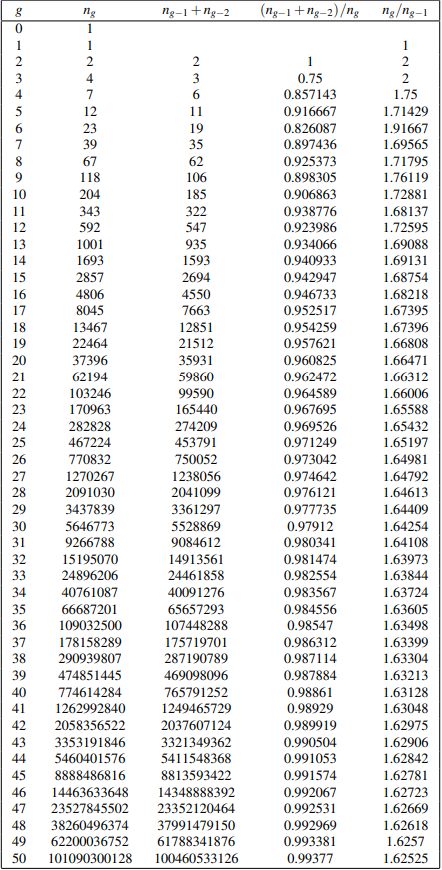
\includegraphics{Erik/Napkin/image.png}
    \caption{Screenshot from Garcia-Sanchez}
    \label{fig:enter-label}
\end{figure}
